\chapter{Deep Learning}
\label{cha:dl}

Machine learning methods are used widely for regression and classification problems. Contemporary companies in order to keep up with the pace of customers expectations rely heavily on such algorithms. They require human intervention to learn. Which is possible for relatively small data sets, but gets extremely complicated or even impossible for larger ones. \textbf{Deep learning (DL)}, however, solves that issue by eliminating the need of human supervision by automating feature extraction. These algorithms can leverage from labeled data sets but do not require them to function. Together with the scalability, DL methods are by far superior to any other Artificial Inteligence solutions. This sections gives an insight of how \textbf{Deep Neural Networks (DNN)}, which are the core of DL, are created.


\section{Neuron}
\label{sec:neuron}

Neuron is the most elementary part of the \textbf{Artificial Neural Network (ANN)}. The idea behind it was to emulate the behaviour of its biological counterpart. It consists of set of inputs $x_1, x_2, ..., x_n$ connected with digital synapses. Each of this connections is given a weight $w_1, w_2, ..., w_n$ representing an importance of the receptive inputs to the output. The output of neuron is determined by the \textbf{activation function} $\phi(x)$, which is described in more detail in the next section (\ref{sub:activation-function}). Where $x$ is the weighted sum of $\sum_j {x_j}{w_j}$ offset by bias $b$. To simplify, the weighted sum can be expressed as a dot product $x \cdot w$.

\begin{figure}[h]
    \centering
    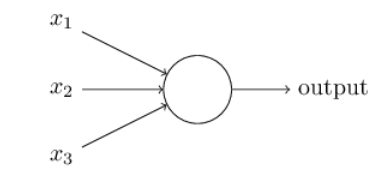
\includegraphics[width=8cm]{img/Perceptron.png}
    \caption{A neuron. Source \cite{NNandDL}}
    \label{fig:neuron}
\end{figure}

\section{Activation Function}
\label{sec:activation-function}

Every neuron in network, except inputs, consists of an activation function. In simple terms, it takes sum of weighted inputs and returns a value which tells how strong the neuron fires. In other words, the higher the activation function return, the stronger influence it has on the next layer. The return is usually within the range $[0, 1]$. Examples of activation functions are: 
\begin{itemize}
    \item Threshold \hspace{5pt}
        $\phi(x) = 
        \begin{cases}
            1 & x \ge 0 \\
            0 & x<0
        \end{cases}$
    \item Sigmoid \hspace{5pt}
        $\phi(x) = \frac{1}{1+e^{-x}}$
    \item Hyperbolic Tangent (tanh) \hspace{5pt}
        $\phi(x) = \frac{1-e^{-2x}}{1+e^{-2x}}$
    \item Rectifier Linear Unit (ReLU) \hspace{5pt}
        $\phi(x) = max(x, 0)$
\end{itemize}

The most commonly used is undoubtedly the \emph{ReLU}, which was proposed and researched by \emph{Xavier Glorot et al.} \cite{DeepSparseReNN}. It allows a network to easily obtain a sparse representation, which has numerous advantages and also mostly resembles neurobiological structures. Human brain is hypothesized to have 95\% to 99\% sparsity.

\section{General architecture of artificial neural network}
\label{sec:general-architecture-ann}

The leftmost layer of the network is called input layer and so are called the neurons that it consist of - \emph{input neurons}. The rightmost output layer consists of, no surprise, \emph{output neurons}. All the in-between layers are called \emph{hidden}. At first glance, the term ``hidden'' may perhaps sound mysterious. However, there is not special meaning behind it. It could be as well called ``not an input or an output'' and be self-explanatory of what it actually is. A network is always made of an input, output and one or more deep layers.

\begin{figure}[h]
    \centering
    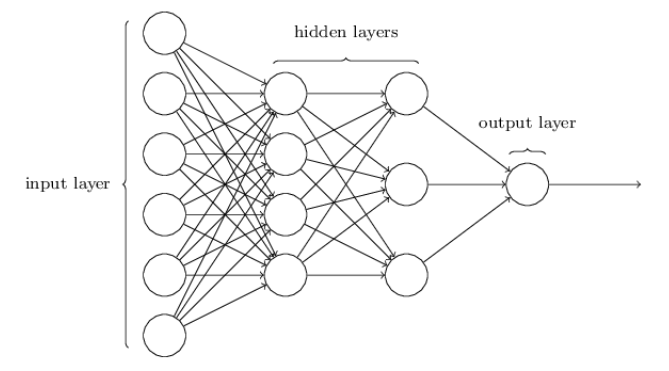
\includegraphics[width=12cm]{img/ANN-diagram.png}
    \caption{An artificial neural network. Source \cite{NNandDL}}
    \label{fig:ann}
\end{figure}

\section{Cost Function}
\label{sec:cost-function}

\subsubsection*{Notation}
\label{sub2:notation}

Before jumping straight into mathematical details, there should be a notation explained so it would not confuse anyone. The one was originally proposed by Michael Nielsen in \emph{Neural networks and deep learning} \cite{NNandDL}.

The \emph{activation} (output) of the $j^{th}$ neuron in the $l^{th}$ layer is called $a^l_j$. Subsequently, the $j^{th}$ element of the input vector would be $a^1_j$. Now we can write down relation between consequent layers outputs:

\begin{equation}
\label{eq:2.1}
a^i_j = \phi\left(\sum_k (w^l_{jk} \cdot a^{l-1}_k) + b^l_j\right)
\end{equation}

where $\phi$ is the activation function,

$w^l_{jk}$ is the weight from the $k^{th}$ neuron in the $(l-1)^{th}$ layer to the $j^{th}$ neuron in the $l^{th}$ layer,

$b^l_j$ is the bias of the $j^{th}$ neuron in the $l^{th}$ layer,

$z^l_j = \sum_k (w^l_{jk} \cdot a^{l-1}_k) + b^l_j$ is the activation value of the neuron before the application of activation function.

For more concise notation we write $a^l = \phi(w^l a^{l-1} + b^l)$, taking advantage of matrix and vector operations.

Having a concise notation, we can discuss what the cost function actually is. Briefly, it is a method of measuring of how good the neural network performed regarding given training sample and the expected output. The return of cost function is always a scalar value, since it indicates overall network performance. It can be written in a form of a following tuple

\[C(W, B, S^r, E^r)\]

where $W$ are network's weights, $B$ biases, $S^r$ is the input of a single training sample and $E^r$ is the desired output of a single training sample.

\subsubsection*{Requirements}
\label{sub2:cost-requirements}

In order to compute gradient, which is a key part of a DNN learning process, the cost function must satisfy following constraints:

\begin{enumerate}
    \item The cost function $C$ must be able to be written as an average
    
        \[C = \frac{1}{n} \sum_x C_x\]
        
        over cost functions $C_x$ for individual training examples $x$.
    
        This property allows to compute a gradient for a single training sample and run \emph{gradient descent}.
    
    \item The cost function $C$ must be independent of any activation values except the output $a^L$.
    The equation for finding the gradient for the output layer only depends on the cost function. Only the following layers are dependent on the next layer. If $C$ was correlated with other activations, it would break the backpropagation algorithm, which will be further described.
\end{enumerate}

\subsubsection*{Examples}
\label{sub2:cost-function-examples}

\begin{enumerate}
    \item \textbf{Mean Squared Error (Quadratic Cost)}
    
    \begin{equation}
        C = \frac{1}{2}\sum_j (a^L_J - E^r_j)^2
    \end{equation}
    
    \item \textbf{Binary Cross-entropy}
    
    \begin{equation}
        C = -\sum_j\left(E_j^rlna_j^L + (1-E_j^r) ln(1 - a_j^L)\right)
    \end{equation}
    
\end{enumerate}

\section{Gradient descent}
\label{sec:gradient-descent}

Imagine a ball rolling down a valley. Intuitively no matter what the starting position is, the ball would eventually end at the bottom. It may roll over the other side, but without any additional force put, it has to find the local minimum. 

This analogy tells what the gradient descent is all about. Applied to greater scale with multiple valleys in a higher dimensional world, but the idea behind remains unchanged. Every neural network is initialized with random weights $W$ and biases $B$, which are fine tuned until the cost function reaches its local (hopefully global) minimum. How it is actually achieved?

To begin with, we need to introduce extremely useful mathematical tool called \emph{gradient}, which is a vector of all partial derivatives of given function. It has a property of always pointing at the direction of the steepest ascent. So in order to find a minimum, we simply need to calculate the negative. For a function $C$ having $x_1, x_2, ..., x_n$ arguments the gradient would be written as 

\begin{equation}
\nabla C = \left(\frac{\partial C}{\partial x_1}, \frac{\partial C}{\partial x_2}, ..., \frac{\partial C}{\partial x_n}\right)^T
\end{equation}

With that definition, there can be computed a step that has to be taken to move value of a function $C$ closer to the minimum:

\begin{equation}
x \longrightarrow x' = x - \eta \nabla C
\end{equation}

where $\eta$ is a small, positive parameter known as \emph{learning rate}.

If this process is done repeatedly, value of $C$ will be decreasing until, hopefully, the global minimum would be reached. The important thing to denote is that $\eta$ has to be small enough not to overshoot, because it would cause the values of a function to diverge, which is the opposite of what we want to achieve. To sum up, the gradient descent algorithm repeatedly computes gradient $\nabla C$ and then moves the return value of a function towards a minimum.

\newpage

For a neural network, a gradient descent is used to find weights $w_k$ and biases $b_l$ which minimize the cost function:

\begin{equation}
    w_k \longrightarrow w_k' = w_k - \eta \frac{\partial C}{\partial w_k}
\end{equation}

\begin{equation}
    b_l \longrightarrow b_l' = b_l - \eta \frac{\partial C}{\partial b_l}
\end{equation}

It would mean that in order to compute a gradient $\nabla C$ we would need to compute $\nabla C_x$ for every training input $x$. For a greater training inputs, it requires immense computational power and causes the learning to significantly slow down. This approach is called \emph{batch learning}, because it takes entire batch of inputs and performs operations on it. In order to avoid that issue, instead of classical gradient descent the \emph{stochastic} version of it is used. The idea is to take a small batch $m$ of randomly chosen training inputs and then perform gradient descent on it. Provided the size $m$ is large enough, the expected average value of $\nabla C_{x_j}$ would be roughly equivalent to the average over all $\nabla C_x$.

\emph{Yann Lecun} in chapter ``Efficient backprop'' in ``Neural Networks: tricks of the trade'' \cite{EfficientBackProp} gives a compact summary of the advantages of stochastic learning:

\begin{itemize}
    \item Stochastic learning is usually much faster than batch learning.
    \item Stochastic learning also often results in better solutions.
    \item Stochastic learning can be used for tracking changes.
\end{itemize}

After the gradient decent for a batch is performed, there is another batch picked from remaining samples. This process is repeated until the training inputs are exhausted, which closes one learning \emph{epoch}.

\section{Backpropagation}
\label{sec:backpropagation}

Before explaining how the algorithm works, let us rewrite \ref{eq:2.1} to vectorized form. Vectorization is the idea of applying given function $f(x)$ to every element of the vector respectively, that is, given that $f(x) = x^3$:

\begin{equation}
    f\left(\begin{bmatrix}
         2 \\
         4 \\
         6
    \end{bmatrix}
    \right) =
    \begin{bmatrix}
        f(2) \\
        f(4) \\
        f(6)
    \end{bmatrix} = 
    \begin{bmatrix}
        8 \\
        64 \\
        196
    \end{bmatrix}
\end{equation}

Having that notation in mind, the equation \ref{eq:2.1} can be written as following:
\begin{equation}
    a^l = \phi \left(w^la^{l-1} + b^l \right)
\end{equation}

Which is much neater version of the same equation, and gives much more global perspective of how the activations of the previous layer affect the next one. It also enables to to avoid indexing hell.
While computing activation, the intermediate value $z^l \equiv w^la^{l-1}+b^l$ is evaluated, which was also described in \ref{sec:cost-function}. It is widely used in a backpropagation so it is worth keeping that in mind.

\vspace{.5cm}

Backpropagation is all about understanding how changing weights and biases in a network affect the cost function. Eventually, it means computing partial derivatives $\frac{\partial C}{\partial w^l_{jk}}$ and $\frac{\partial C}{\partial b^l_j}$. In order to compute them, the intermediate value $\delta^l_j$ has to be introduced. It is called an \emph{error} int the \emph{j-th} neuron of the \empth{l-th} layer and is computed in a backpropagation algorithm and then related to desired partial derivatives of weights and biases.

\begin{equation}
    \delta^l_j \equiv \frac{\partial C}{\partial z^l_j}
\end{equation}

The error is a measure of how the change in the weighted input of an activation function changes the cost function.

There are four fundamental equations on which backpropagation is founded.

\subsubsection*{Error in the output layer $\delta^L$}
\label{sub2:error-in-the-output-layer}

The components of $\delta^L$ is in form:

\begin{equation}
\delta^L_j = \frac{\partial C}{\partial a^L_j}\phi'(z^L_j)
\tag{EQ1}
\label{eq:bp-eq1}
\end{equation}

This expression consists of two elements. First one $\frac{\partial C}{\partial a^L_j}$ tells how fast the cost is changing with respect to \emph{j-th} output activation. The latter $\phi'(z^L_j)$ tells how fast the activation function is changing at $z^L_j$.

\ref{eq:bp-eq1} can be rewritten to matrix form as

\begin{equation}
    \delta^L = \nabla_a C \odot \phi'(z^L)
    \tag{EQ1a}
    \label{eq:bp-eq1a}
\end{equation}

Where $\nabla_a C$ is a vector of all partial derivatives $\frac{\partial C}{\partial a^L_j}$ and $\odot$ is a operation of element-wise vector multiplication.

\subsubsection*{Error $\delta^l$ in terms of the error in the next layer $\delta^{l+1}$}
\label{sub2:delta-l-to-delta-l+1}

\begin{equation}
    \delta^l = \left((w^{l+1})^T\delta^{l+1}\right) \odot \phi'(z^l)
    \tag{EQ2}
    \label{eq:bp-eq2}
\end{equation}

At a first glance this equation may seem complicated, but it has an extremely intuitive interpretation. Assuming the $\delta^{l+1}$ is a known value, applying $(w^l+1)^T$ can be understood as moving the error \emph{backward} through the network, giving the measure of the output error or the \emph{l-th} layer. Taking the element-wise product with $\phi'(z^l)$ moves the error backward through the activation function of neuron in layer $l$ resulting in the error $\delta^l$ in the weighted input of layer $l$.

Using \ref{eq:bp-eq1} and \ref{eq:bp-eq2} one can compute any error $\delta^l$ in the network.

\subsubsection*{Rate of change of the cost with respect to any bias of the network}
\label{sub2:rate-of-change-of-the-cost-with-respect-to-every-bias-of-the-network}

\begin{equation}
    \frac{\partial C}{\partial b} = \delta
    \tag{EQ3}
    \label{eq:bp-eq3}
\end{equation}

This is a shorthand notation with the assumption that error $\delta$ is evaluated at the same neuron as the bias $b$.

\subsubsection*{Rate of change of the cost with respect to any weight in the network}
\label{sub2:rate-of-change-of-the-cost-with-respect-to-any-weight-in-the-network}

\begin{equation}
    \frac{\partial C}{\partial w} = a_{in} \delta_{out}
    \tag{EQ4}
    \label{eq:bp-eq4}
\end{equation}

Where $a_{in}$ is understood as an activation of the neuron input to the weight $w$ and $\delta_{out}$ is the error of the neuron output from the same weight $w$. Notice when the activation is small $a_{in} \approx 0$ then the gradient term $\frac{\partial C}{\partial w}$ is also small. Therefore the weight changes in a slow pace during gradient descent. In other words, the weight \emph{learns slowly}.


\subsubsection*{Algorithm}
\label{sub2:bp-algorithm}

Having introduced all the necessary equations, the algorithm presents in a following way, as described in ``Neural Networks and Deep Learning'' by \emph{Michael Nielsen} \cite{NNandDL}.

\begin{enumerate}
    \item \textbf{Input} $x$: Set the corresponding activation $a^1$ of the input layer.
    \item \textbf{Feedforward}: For each $l = 2, 3, ..., L$ compute $z^l = w^la^{l-1}+b^l$ and $a^l$.
    \item \textbf{Output error} $\delta^L$: Compute the vector $\delta^L = \nabla_a C \odot \phi'(z^l)$.
    \item \textbf{Backpropagate the error}: For each $l = L-1, L-2, ..., 2$ compute 
        $\delta^l = \left((w^{l+1})^T \delta^{l+1}\right) \odot \phi(z^l)$
    \item \textbf{Output}: The gradient of a cost function is given by 
        $\frac{\partial C}{\partial w^l_{jk}} = a^{l-1}_k \delta^l_j$ 
        and 
        $\frac{\partial C}{\partial b^l_j} = \delta^l_j$
\end{enumerate}

By now it should be clear why this algorithm is called backpropagation. It takes cost function, that is a function of outputs of a network, as an input to compute the error of the output layer and then propagates the errors backwards.